
\documentclass[margin]{res}  
\textheight=700pt

\usepackage{graphicx}
\graphicspath{ {./} }

\begin{document}

\begin{minipage}{0.35\linewidth}
    \begin{center}
        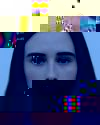
\includegraphics[width=0.9\linewidth]{photo}
    \end{center}
\end{minipage}
\hfill
\begin{minipage}{0.85\linewidth}
\textbf{Volha Andrava\\}
\textbf{ola.androva@gmail.com \\(+48) 795084463\\}
\end{minipage}
\begin{resume}

\section{OBJECTIVE}
{\sl Second year  student at Adam Mickiewicz University. Goal oriented, hard-working and responsible. I had practical experience with many popular programming languages. }


\section{EDUCATION}
\textbf{Adam Mickiewicz University}, Poznan\\
{\sl Bachelor of Computer Science }\\
Expected January, 2023

\textbf{Gymnasium № 23} (Belarus, Minsk) \\
2008-2019

\textbf{Computer Academy ITStep}, (Belarus, Minsk) \\
2018-2019

\section{LANGUAGES}

\begin{itemize}
    \item Russian (Native)
    \item Belorussian (Native)
    \item English (B2)
    \item Polish (Pre-Intermediate)
\end{itemize}

\section{TECHNICAL\\SKILLS}

\textbf{Languages : } Python, C++, C, Pascal
\\
\textbf{Familiar : } Javascript, HTML, CSS
\\
\textbf{General : } Algorithms and Data Structures, Object Oriented Programming


\section{OPERATING SYSTEMS}
\textbf{Windows, Mac OS, Linux  \\}

\section{PROJECTS}
\title{\textbf{Microshell\hfill Dec 2019}
 }
\begin{position}
Shell program written using ANSI C language.The program accepts  commands as input and then performs actions in accordance with their content. 
%\begin{itemize}
\item \textbf{Technology/Tools:} ANSI C
%\end{itemize}
\end{position}


\title{\textbf{Mockup for a web page \hfill Dec 2019}
 }
\begin{position}
The task was to develop mockup for a main page of a modern newspaper. Using at least 30 different resources.
%\begin{itemize}
\item \textbf{Technology/Tools:} HTML, CSS
%\end{itemize}
\end{position}


\section{RELEVANT\\COURSES}
\par

\normalfont{\textbullet{} Fundations of Programming\\ }
\normalfont{\textbullet{} Algorithms and Data Structures\\ }
\normalfont{ \textbullet{} Introduction to Computer Science \\}
\normalfont{\textbullet{} Operating System\\}
\normalfont{\textbullet{} Introduction to mathematics\\}

\section{ADDITIONAL COURSES\\IN "COHERENT SOLUTIONS"}

\normalfont{ \textbullet{} Python(2017) Algorithms and Data Structures(2018) \\}
\normalfont{ \textbullet{} Algorithms and Data Structures(2018) \\}
\normalfont{\textbullet{} JavaScript(2019)\\ }



\end{resume}
\(\)\end{document}